\documentclass[twoside,twocolumn]{article}

\usepackage{blindtext} % Package to generate dummy text throughout this template 
\usepackage{graphicx}
\usepackage[sc]{mathpazo} % Use the Palatino font
\usepackage[T1]{fontenc} % Use 8-bit encoding that has 256 glyphs
\linespread{1.05} % Line spacing - Palatino needs more space between lines
\usepackage{microtype} % Slightly tweak font spacing for aesthetics

\usepackage[english]{babel} % Language hyphenation and typographical rules

\usepackage[hmarginratio=1:1,top=32mm,columnsep=20pt]{geometry} % Document margins
\usepackage[hang, small,labelfont=bf,up,textfont=it,up]{caption} % Custom captions under/above floats in tables or figures
\usepackage{booktabs} % Horizontal rules in tables
\usepackage{graphicx}
\usepackage{lettrine} % The lettrine is the first enlarged letter at the beginning of the text

\usepackage{enumitem} % Customized lists
\setlist[itemize]{noitemsep} % Make itemize lists more compact

\usepackage{abstract} % Allows abstract customization
\renewcommand{\abstractnamefont}{\normalfont\bfseries} % Set the "Abstract" text to bold
\renewcommand{\abstracttextfont}{\normalfont\small\itshape} % Set the abstract itself to small italic text

\usepackage{titlesec} % Allows customization of titles

\titleformat{\section}[block]{\large\scshape\centering}{\thesection.}{1em}{} % Change the look of the section titles
\titleformat{\subsection}[block]{\large}{\thesubsection.}{1em}{} % Change the look of the section titles

\usepackage{fancyhdr} % Headers and footers
\pagestyle{fancy} % All pages have headers and footers
\fancyhead{} % Blank out the default header
\fancyfoot{} % Blank out the default footer
\fancyhead[C]{Data Story Telling Examples$\bullet$ Marzo 2022 $\bullet$ } % Custom header text
\fancyfoot[RO,LE]{\thepage} % Custom footer text

\usepackage{titling} % Customizing the title section

\usepackage{hyperref} % For hyperlinks in the PDF

%----------------------------------------------------------------------------------------
%	TITLE SECTION
%----------------------------------------------------------------------------------------
\providecommand{\keywords}[1]{
  \small	
  \textbf{\textit{\quad \quad Keywords: }} #1}

\providecommand{\pclave}[1]{
  \small	
  \textbf{\textit{\quad \quad Palabras Clave: }} #1}

%Idiomas: \selectlanguage{english} \selectlanguage{spanish}

\begin{document}

\title{Trabajo Encargado N°2: Data Story Telling Examples}

\begin{titlepage}
\begin{figure}[htb]
\begin{center}

\includegraphics[width=5cm]{imagenes/logo.png}
\end{center}
\end{figure}
\vspace*{-0.25in}
\begin{center}
\large{UNIVERSIDAD PRIVADA DE TACNA}\\
\vspace*{-0.025in}
INGENIERIA DE SISTEMAS  \\	

\vspace*{0.5in}
\begin{large}
TITULO:\\
\end{large}

\vspace*{0.1in}
\begin{Large}
\textbf{Data Story Telling Examples} \\
\end{Large}

\vspace*{0.3in}
\begin{Large}
\textbf{CURSO:} \\
\end{Large}

\vspace*{0.1in}
\begin{large}
Inteligencia de Negocios\\
\end{large}

\vspace*{0.3in}
\begin{Large}
\textbf{DOCENTE:} \\
\end{Large}

\vspace*{0.1in}
\begin{large}
 Ing. Patrick Cuadros Quiroga\\
\end{large}

\vspace*{0.2in}
\vspace*{0.1in}
\begin{large}

Integrantes: \\
\begin{flushleft}
Maldonado Cancapi, Carlos Alejandro\hfill(2018000660) \\
Huillca Aroni, Alfredo\hfill(2018060903)\\
Anahua Huayhua, Jenny Karen\hfill(2018062150)\\
Coloma Colquehuanca, Kiara\hfill(2018062218)\\

\end{flushleft}
\end{large}

\vspace*{0.1in}
\begin{large}
Tacna - Perú\\
2022
\end{large}
\end{center}
\end{titlepage}

\setlength{\droptitle}{-4\baselineskip} % Move the title up

\pretitle{\begin{center}\Huge\bfseries} % Article title formatting
\posttitle{\end{center}} % Article title closing formatting
\title{ Data Story Telling Examples } % Article title

\date{\today} % Leave empty to omit a date                     
\renewcommand{\maketitlehookd}{%

}

%----------------------------------------------------------------------------------------



% Print the title
\maketitle

%----------------------------------------------------------------------------------------
%	ARTICLE CONTENTS
%----------------------------------------------------------------------------------------

\section{Resumen}
Estamos acostumbrados   a   tablas   dinámicas   y ahora,   
las   nuevas herramientas de visualización de datos como 
Tableau o Qlikview tienen mucha aceptación  porque  puedes  jugar  con  los  
datos,  ver como cambian las previsiones o los resultados según combinas 
las variables. Todo con colores y muy vi- sual. Vamos, que queda muy chulo 
ver un cuadro de mandos con colorines y mapas en 3D y todo eso, pero nos 
encontraremos con un problema gordo y es que, según en un 
post previo las empresas que están invirtiendo en analítica predictiva 
(integrar difer- entes datos para predecir el mercado) siguen teniendo 
problemas a la hora de desarrollar acciones para los insights que les están 
dando los diferentes algoritmos.
 
Esto  no  es  mas  que,  pese  a  que  tienen  
buenos datos,  no  entienden  bien  lo  que  los  datos les  están  
contando.   Y  he  aquí  la  solución:   
hacer de los datos algo con lo que la persona de negocio sienta relación.  
Aquí entra, ni más ni menos que el denominado Storytelling con datos o 
historias que generen un impacto o un cambio en las acciones de una 
persona basado en los resultados de un análisis. En las antiguas 
civilizaciones, los jefes de los pueblos  realizaban  preguntas  a  los  
oráculos  para poder   saber   qué  hacer   
(invadir   un   pueblo   cer- cano, responder o no a 
las amenazas de otros diri- gentes. . . )	Luego,   los   oráculos   
(no   sabemos   si puestos  hasta  arriba  de  algún  alucinogeno)  
daban respuestas de lo más 
creativas que dejaba al jefe con los deberes de interpretar lo que el oraculo había 
dicho.


%------------------------------------------------

\section{Abstract}

We are used to dynamic tables and now, the new data visualization tools such as Tableau or Qlikview have a lot of acceptance because you can play with the data, see how the forecasts or the results change as you combine the variables. All with colors and very visual. Come on, it is very cool to see a dash- board with 3D colors and maps and all that,  but we will find a big problem and that is, according to a previous post the companies that are invest- ing in predictive analytics (integrate different data to predict the market) continue to have problems when developing actions for the insights that the different algorithms are giving them.
This is nothing more than, although they have super cool data, they don’t understand well what the data is telling them. And here is the solution: make the data something with which the business person feels relationship. Here he enters, neither more nor less than the so-called Storytelling with data or stories that generate an impact or a change in the actions of a person based on the results of an analysis.
In ancient civilizations, village chiefs asked the oracles questions so they could know what to do (in- vade a nearby town, respond or not to the threats of other leaders ...) Then, the oracles (we don’t know if they are placed up to some hallucinogenic) gave answers as creative as he left the boss with the duties of interpreting what the oracle had said.






%------------------------------------------------
\section{Introduccion}
La Narrativa en la Visualización de Datos es una
de las principales herramientas del Big Data que
los negocios no se pueden perder.Por eso, en este
post te contamos lo más interesante del DataStorytelling, qué es y cómo mejorar los resultados
gracias a ello.

Cada vez se van a necesitar más profesionales big data y storytelleres en
el sector. El cambio en la era digital demanda
perfiles con capacidades analiticas y de inteligencia
empresarial. Como consecuencia, las nuevas
generaciones irán más allá de estas disciplinas, con
nuevas ideas y espacios para los negocios.

\begin{center}

\end{center}

\section{Desarrollo}


\subsection{Concepto}
La narración de datos (data storytelling) 
es el concepto de construir una narrativa 
convincente basada en datos y análisis 
complejos que ayudan a respaldar el mensaje 
de su historia para influir e informar a 
una audiencia en particular. La narración 
de datos es muy similar a la narración humana, 
pero brinda los beneficios adicionales de conocimientos más profundos y evidencia de respaldo a través de gráficos y tablas. La narración de datos efectiva también puede:
\begin{itemize}
    \item   Ayude a las empresas a conocer los deseos y necesidades de su audiencia. 
    \item   Elimine las exposiciones de riesgo a procesos desconocidos. 
    \item   Proporcionar credibilidad como líder de pensamiento de la industria y el tema. 
\end{itemize}

A través de la narración de datos, 
la información complicada se simplifica 
para que su audiencia pueda interactuar 
con su contenido y tomar decisiones críticas 
de manera más rápida y segura.


\subsection{Beneficios}
\begin{itemize}
    \item   Añade valor a los datos y conocimientos. 
    \item   Interpreta información compleja y resalta puntos clave esenciales para la audiencia. 
    \item   Aporta un toque humano a sus datos.
    \item   Ofrece valor e influencia potencial para su audiencia e industria.
\end{itemize}

\subsection{Pasos para crear una historia}

\begin{itemize}
    \item   Piensa en tu teoría. ¿Qué quieres probar o refutar? ¿Qué crees que te dirán los datos?
    \item   Recolectar datos. Recopile los datos que necesitará para desarrollar su historia. 
    \item   Define el propósito de tu historia. Usando los datos que reuniste, deberías poder escribir cuál es el objetivo de tu historia en una sola oración. 
    \item   Piensa en lo que quieres decir. Resume todo, desde la introducción hasta la conclusión 
    \item   Hacer preguntas. ¿Estabas en lo correcto o equivocado en tu hipótesis? ¿Cómo dan forma estas respuestas a la narrativa de su historia de datos? 
    \item   Crea un objetivo para tu audiencia. ¿Qué acciones le gustaría que tomaran después de leer su historia?
\end{itemize}

\subsection{Visualizacion de datos}
La visualización de datos juega un papel importante en 
la determinación de cuán receptiva es su audiencia 
para recibir información compleja. La visualización 
de datos ayuda a transformar cantidades ilimitadas de 
datos en algo más simple y digerible. Aquí, puede 
proporcionar las imágenes necesarias para respaldar 
su historia. Las visualizaciones de datos efectivas 
pueden ayudar a:
\begin{itemize}
    \item   Revela patrones, tendencias y hallazgos desde un punto de vista imparcial. 
    \item   Proporcione contexto, interprete resultados y articule ideas. 
    \item   Agilice los datos para que su audiencia pueda procesar la información.
    \item   Mejorar la participación de la audiencia.
\end{itemize}

\subsection{Elementos claves de la narración de datos}
A través de un enfoque estructurado, la narración de datos y 
la visualización de datos trabajan juntos para comunicar sus 
conocimientos a través de tres elementos esenciales: narración, 
imágenes y datos. A medida que crea su historia de datos, es 
importante combinar los siguientes tres elementos para escribir 
una anécdota completa de su teoría y las acciones resultantes que 
le gustaría ver de los usuarios con los datos de apoyo.

\begin{itemize}
    \item \textbf{Construye tu narrativa}
    
    A medida que cuente su historia, necesita usar sus datos como pilares de apoyo para sus conocimientos. Ayude a su audiencia a comprender su punto de vista destilando información compleja en conocimientos informativos. Su narrativa y contexto son lo que impulsará la naturaleza lineal de su narración de datos.
    \item \textbf{Usa imágenes para iluminar}
    
    Las imágenes pueden ayudar a educar a la audiencia sobre su teoría. Cuando conecta los activos visuales (tablas, gráficos, etc.) a su narrativa, involucra a la audiencia en conocimientos ocultos con los datos fundamentales para respaldar su teoría. En lugar de presentar una única perspectiva de datos para respaldar su teoría, es útil mostrar múltiples datos, tanto granulares como de alto nivel, para que la audiencia pueda apreciar verdaderamente su punto de vista.
    \item \textbf{Mostrar datos para apoyar}
    
    Las imágenes pueden ayudar a educar a la audiencia sobre su teoría. Cuando conecta los activos visuales (tablas, gráficos, etc.) a su narrativa, involucra a la audiencia en conocimientos ocultos con los datos fundamentales para respaldar su teoría. En lugar de presentar una única perspectiva de datos para respaldar su teoría, es útil mostrar múltiples datos, tanto granulares como de alto nivel, para que la audiencia pueda apreciar verdaderamente su punto de vista.
\end{itemize}
\subsection{Herramientas para elaborar data storytelling}

\subsubsection{Análisis guiado}
Estas soluciones combinan la visualización de datos exploratorios con texto explicativo y elementos gráficos. Las aplicaciones interactivas de narración de datos creadas por estas plataformas pretenden ser una alternativa a los paneles e informes tradicionales.


\textbf{Juicebox}

Juicebox combina un estilo moderno de periodismo de datos con visualizaciones exploratorias que se conectan automáticamente para permitir el análisis. Un enfoque en la creación fácil hace de Juicebox la única herramienta en esta categoría que es accesible para usuarios no técnicos o no analistas.

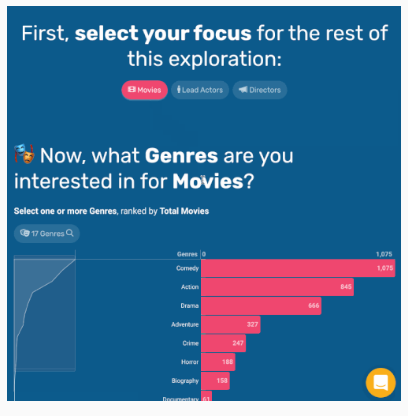
\includegraphics[width=7cm]{imagenes/img1.png}

\textbf{Toucan toco}

Esta plataforma está dirigida a compradores empresariales y tiene un enfoque único para presentar historias de datos. El uso compartido, la anotación y las vistas detalladas de la historia le brindan la oportunidad de comunicar una descripción general completa de un tema. 

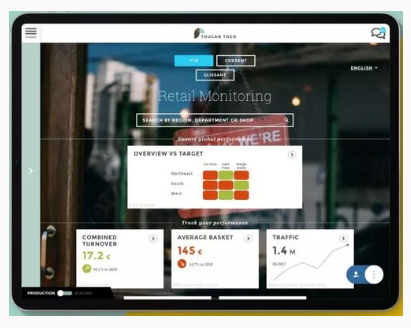
\includegraphics[width=7cm]{imagenes/img2.png}


\textbf{Nugit}


Nugit ha pasado desapercibido para algunos clientes, pero representa una de las soluciones de narración de datos más completas del mercado. El diseño atractivo combinado con potentes funciones de texto hacen de esta una solución que vale la pena ver. 


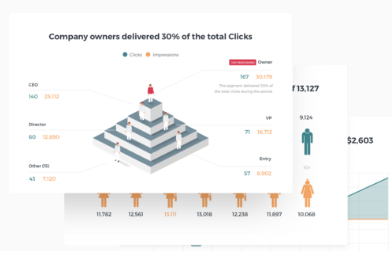
\includegraphics[width=7cm]{imagenes/img3.png}



\subsubsection{Narración de datos como característica} 
Este conjunto de soluciones son plataformas integrales de inteligencia empresarial y análisis visual. La narración de datos se presenta como una característica o técnica que se puede lograr dentro de la plataforma más grande.

Tableau, líder en análisis visual, vio el potencial de la narración de datos desde el principio. Lanzaron una función llamada 'Story Points' en 2014. La función no ha logrado una amplia adopción entre su base de clientes y Tableau parece estar centrándose en las opciones de exportación de PowerPoint.

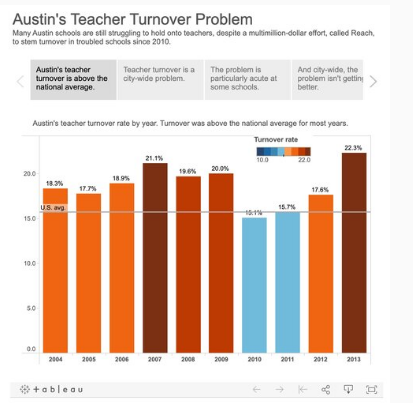
\includegraphics[width=7cm]{imagenes/img4.png}

ArcGis Story Maps: Construida sobre la plataforma de mapeo profundamente establecida, la función StoryMaps permite crear descripciones narrativas para ayudar a los lectores a navegar por una historia enfocada geográficamente.

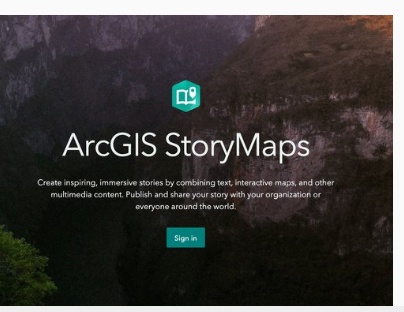
\includegraphics[width=7cm]{imagenes/img5.png}

Historias de Qlik Sense
Qlik Sense es una plataforma de análisis bien establecida con sólidas capacidades de visualización. Si bien recibe menos publicidad que sus competidores Tableau y PowerBI, Qlik comprende la necesidad de llegar a audiencias más amplias en la empresa a través de la narración de datos.

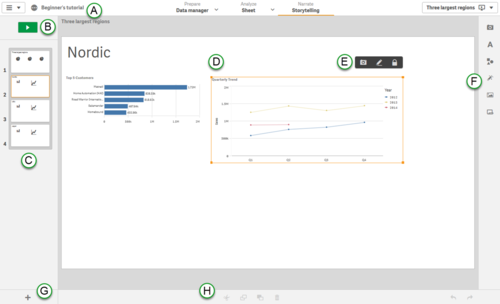
\includegraphics[width=7cm]{imagenes/img6.png}

PowerBI
PowerBI es la respuesta de Microsoft al éxito de la potencia de análisis visual Tableau. Al igual que las otras soluciones de esta categoría, PowerBI brinda orientación, funciones e instrucciones sobre la narración de datos sin brindar una solución enfocada para los usuarios. 

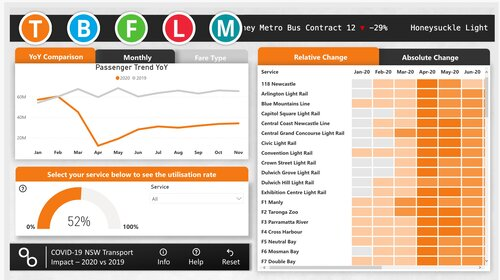
\includegraphics[width=7cm]{imagenes/img7.png}



\subsubsection{Diseño sobre datos}
Estas soluciones para diseñadores se centran en la creación de infografías y presentaciones que pueden incluir tablas y gráficos como parte del documento. Los datos son uno de los muchos elementos de los medios que cuentan la historia.

Infogram: Infogram es una plataforma de diseño flexible que incluye capacidades para agregar gráficos ligeros. Ofrece una variedad de formatos para presentar información, que incluye todo, desde tableros e informes hasta publicaciones y carteles en redes sociales.

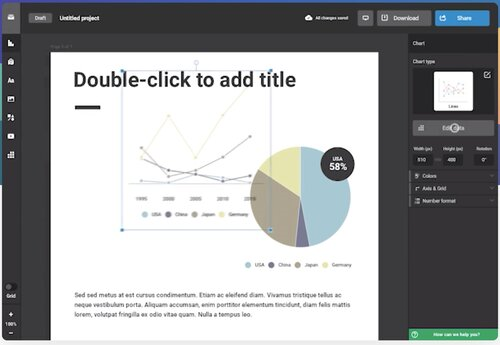
\includegraphics[width=7cm]{imagenes/img8.png}

Vismos
Al igual que las otras herramientas de diseño primero, los gráficos están destinados a mostrar algunos puntos de datos en lugar de permitir el análisis. Tiene una amplia colección de iconos y widgets. 

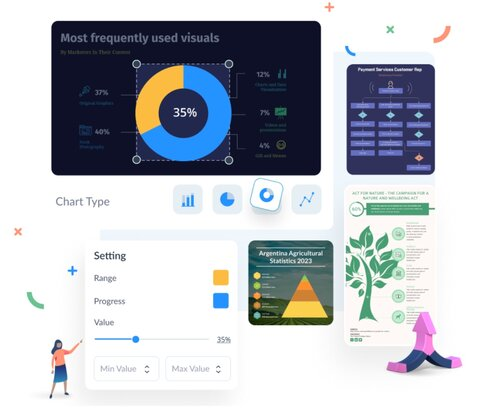
\includegraphics[width=7cm]{imagenes/img9.png}

\subsection{Importancia}

Los datos se recopilan y comparten para ayudarnos a ver patrones y obtener información que de otro modo no tendríamos.

Por ejemplo:
\begin{itemize}
    \item Puede ver las calificaciones de sus estudiantes para ver cómo les está yendo en la escuela.
    \item Su médico puede observar su análisis de sangre para hacer recomendaciones para su estilo de vida.
    \item Su empresa puede observar los cambios en los ingresos para determinar qué tan bien están funcionando las nuevas estrategias comerciales.
    
\end{itemize}

\subsection{Ejemplos de  data storytelling }

Spotify

En los últimos años, Spotify, una aplicación de música, ha enviado resúmenes anuales a sus clientes en formato de correo electrónico. Estas historias cortas extraen estadísticas interesantes para cada usuario, como la cantidad de minutos que han escuchado música en su aplicación. Esta es una forma atractiva de comunicar el valor de su servicio en lugar de simplemente enviarles una factura o un simple agradecimiento por utilizarnos.
Cómo será África dentro de 100 años

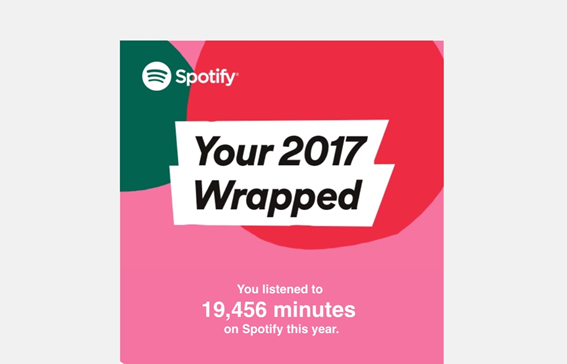
\includegraphics[width=7cm]{imagenes/img10.png}


Cómo será África dentro de 100 años

En algunas historias, los números son tan marcados que deben ocupar un lugar central. Esto es especialmente cierto en esta clásica historia de datos de The Telegraph . 
Con una animación de imágenes estáticas bien ejecutada y basada en desplazamiento, el equipo muestra las implicaciones del rápido crecimiento de la población en todo el continente africano durante el próximo siglo.

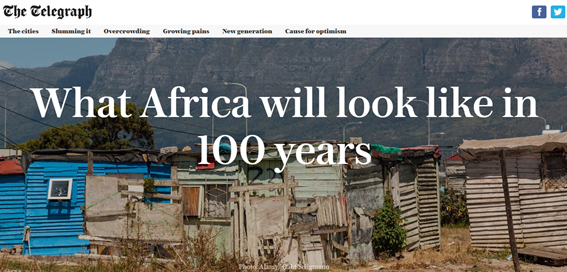
\includegraphics[width=7cm]{imagenes/img11.png}
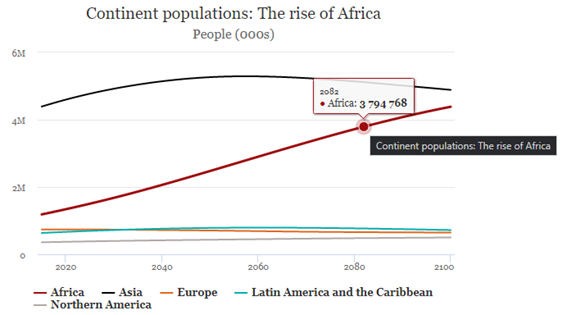
\includegraphics[width=7cm]{imagenes/img12.png}

Cronología del coronavirus

Con el estallido de la pandemia de COVID-19, los equipos de contenido de organizaciones de todo el mundo, incluidas empresas de medios, ONG, universidades y otras empresas, publicaron una gran cantidad de excelentes visualizaciones de datos. Una historia provino de Radio NZ que publicó, y continuó actualizando, una línea de tiempo sobre el impacto de COVID-19 en Aotearoa, Nueva Zelanda . En lugar de usar animación basada en desplazamiento, el equipo de Radio NZ decidió incorporar visualizaciones enriquecidas de la plataforma de visualización de datos 


\includegraphics[width=7cm]{imagenes/img13.png}

Tableau. 

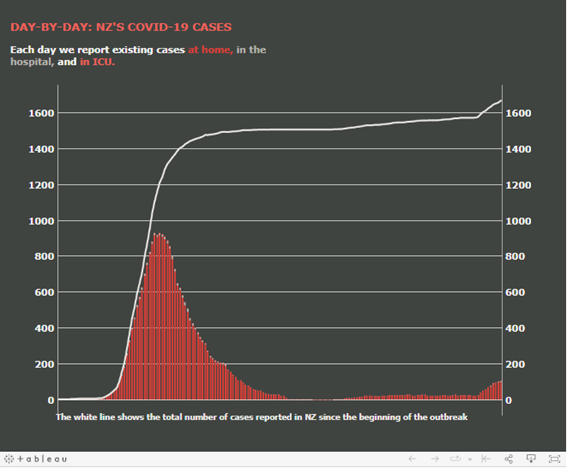
\includegraphics[width=7cm]{imagenes/img14.png}

\section{Conclusiones}
La narración de datos es una metodología útil para comunicar información adaptada a una audiencia de manera específica. La cantidad de datos creados por corporaciones en todo el mundo crece cada año, y gracias a innovaciones como la Internet de las cosas, este crecimiento no muestra signos de disminuir. El problema para las empresas es que estos datos solo son útiles si se pueden extraer de ellos información valiosa y aplicarla.
Data Storytelling va más allá de la representación gráfica de datos, y abarca la combinación de varios elementos claves como son: datos, imágenes y narrativa.
El storytelling es la forma de presentar algo, una historia que está orientada al propósito del marketing, por lo que, como una buena presentación, debe contener un principio, un medio y un final.
teniendo en considerancion el Storytelling, contar la historia de datos es muy similar: parte de una situcacion existente, de que cierta manera es conocida o se conecta con la experiencia de la audiencia, luego cuenta lo que ha pasado para finalmente, llegar a una conclusion



\section{Recomendaciones}
Como seres humanos estamos naturalmente conectados para contar historias como un medio en el cual se comparte de igual manera información. Hoy en día, con la gran cantidad de datos disponibles, únicamente la narración de datos es lo que le puede poner una perspectiva humana al mundo de la era digital cambiante. La influencia en las presentaciones empresariales y financieras, que son entornos objetivos y complejos, requiere una estrategia narrativa y un flujo de información diferentes a los de un comercial o una presentación en otros ámbitos.
Desafortunadamente existen negocios que aún no han podido aprovechar por completo las oportunidades escondidas en sus datos enfrentándose a limitaciones como:
\begin{itemize}
    \item Los informes manuales siguen siendo frecuentes. 
    \item Carecen del componente vital de la narrativa para comunicar de manera efectiva información e ideas.
    \item La mayoría de los equipos de marketing, ventas, operaciones y análisis carecen de los recursos y el tiempo para responder a todas las solicitudes de informes de todos los niveles de una empresa, incluidas las partes interesadas externas, al igual que los clientes.
    \item Puesto de manera simple, los datos en los tableros y los informes únicamente te dicen que está pasando, no te dicen por qué sucede.
\end{itemize}
“La narrativa sumada a los datos hace que la audiencia comprenda de un modo adecuado qué dicen estos números. La suma del componente visual a los datos hace que la atención del usuario capte detalles que de otro modo podría ignorar”. Brent Dykes, en Forbes.



%----------------------------------------------------------------------------------------
%	REFERENCE LIST
%----------------------------------------------------------------------------------------

\begin{thebibliography}{XXX0000}
    \bibitem - What is Data Storytelling | Microsoft Power BI. (2022). Retrieved March 29, 2022, from Microsoft.com website: https://powerbi.microsoft.com/en-za/data-storytelling/
    \bibitem - Data Storytelling: How to Tell a Story With Data - Venngage. (2021, February 18). Retrieved March 29, 2022, from Venngage website: https://venngage.com/blog/data-storytelling/ 
    \bibitem - Nugit. (2013). Retrieved March 29, 2022, from Nugit.co website: https://www.nugit.co/what-is-data-storytelling/
    \bibitem - McGregor, M. (2021, March 7). 8 examples of powerful data storytelling. Retrieved March 29, 2022, from Shorthand.com website: https://shorthand.com/the-craft/examples-of-powerful-data-storytelling/index.html
    \bibitem - Kirk, A. (2016, March 11). What Africa will look like in 100 years. Retrieved March 29, 2022, from Telegraph.co.uk website: http://s.telegraph.co.uk/graphics/projects/Africa-in-100-years/index.html
    \bibitem - Nussbaumer, C. (2015) storytelling with data a data visualization guide for business professionals retrieved from  http://www.bdbanalytics.ir/media/1123/storytelling-with-data-cole-nussbaumer-knaflic.pdf
    \bibitem - Gemignani, Z. (2022, February 16). Data Analytics and Visualization Made Easy - Juice Analytics. Retrieved March 29, 2022, from Data Analytics and Visualization Made Easy - Juice Analytics website: https://www.juiceanalytics.com/writing/best-data-storytelling-solutions
    \bibitem - Gemignani, Z. (2022, February 18). Data Analytics and Visualization Made Easy - Juice Analytics. Retrieved March 29, 2022, from Data Analytics and Visualization Made Easy - Juice Analytics website: https://www.juiceanalytics.com/writing/20-best-data-storytelling-examples
    \bibitem - Data Storytelling: How to Tell a Story With Data - Venngage. (2021, February 18). Retrieved March 29, 2022, from Venngage website: https://venngage.com/blog/data-storytelling/ 
    \bibitem -  Kirk, A. (2016, March 11). What Africa will look like in 100 years. Retrieved March 29, 2022, from Telegraph.co.uk website: http://s.telegraph.co.uk/graphics/projects/Africa-in-100-years/index.html

  

\end{thebibliography}

%----------------------------------------------------------------------------------------

\end{document}\documentclass[twoside,twocolumn]{article}
